\section{Motivating Examples}


\begin{figure*}[t]
  \centering
  \begin{subfigure}[b]{.3\linewidth}
      \centering
      %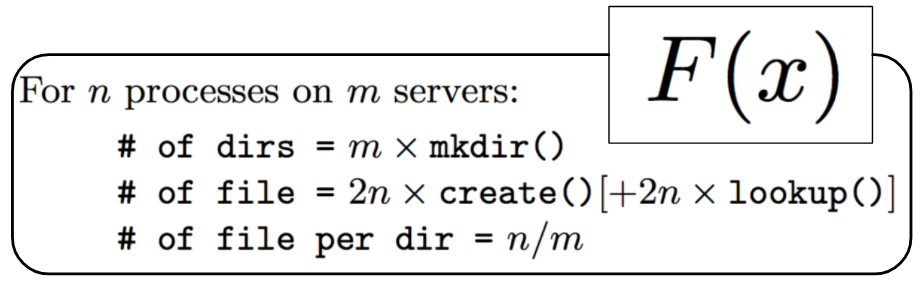
\includegraphics[width=1.0\linewidth]{figures/file-type-formula.png}
For \(n\) processes on \(m\) servers:

\begin{itemize}
  \item[] \texttt{\# of dirs =} \(m \times \texttt{mkdir()}\)
  \item[] \texttt{\# of file =} \(2 \times n \times m\)
  \item[] \texttt{\# of file per dir =} \(n/m\)
\end{itemize}
      \caption{Function for PLFS subtrees.} \label{fig:plfs}
  \end{subfigure}
  \begin{subfigure}[b]{.3\linewidth}
      \centering
      %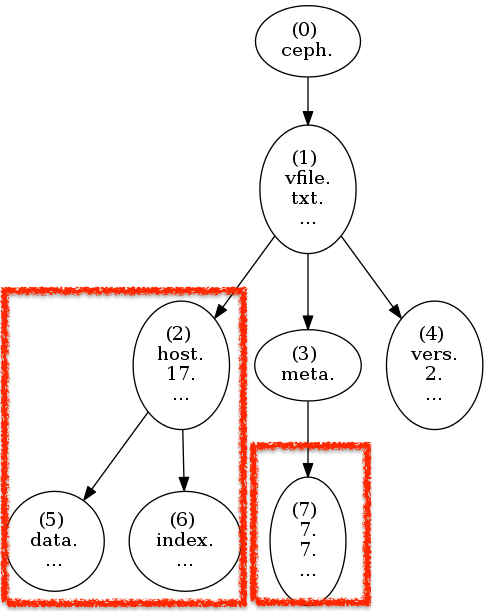
\includegraphics[width=1.0\linewidth]{figures/tree_plfs.png}
      \footnotesize
      %\begin{minted}[xleftmargin=1em,linenos]{c++}
      \begin{minted}[xleftmargin=1em]{c++}
void recurseBranch(TObjArray *o) {
  TIter i(o); 
  for(TBranch *b=i.Next(); i.Next()!=0; b=i.Next()){
    // process branch
    recurseBranch(b->GetListOfBranches());
  }
      \end{minted}
      \caption{Binary for HEP subtrees.} \label{fig:plfs}
  \end{subfigure}
  \begin{subfigure}[b]{.3\linewidth}
      \centering
      %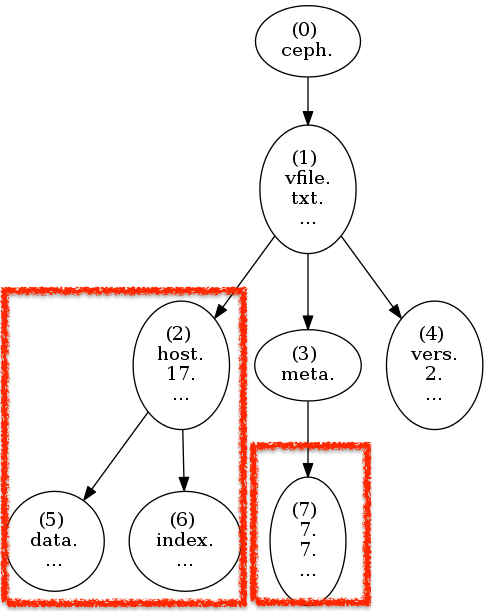
\includegraphics[width=1.0\linewidth]{figures/tree_plfs.png}
      \caption{PLFS} \label{fig:plfs}
  \end{subfigure}
\caption{Namespaces generated by 3 motivating examples.\label{fig:use-cases}}
\end{figure*}

%char *tn = getTreeName().c_str();
%TTree* t = (TTree*) root->Get(tn);
%TIter i(t->GetListOfBranches());
%for(TBranch *b = i.next();
%    i.Next() != 0;
%    b = (TBranch*) i.Next())
%  recurseBranch(b->GetListOfBranches());

To motivate implied namespaces, we look at the namespaces of 3 applications.
Each is from different domains and this list is not meant to be exhaustive, as
similar organizations exist for many domains, even something as distant as the
mail application on a Mac. For scalability reasons, we focus on large scale
systems in high performance computing (HPC) and high energy physics (HEP).

\subsection{PLFS (HPC)}
\label{sec:plfs}
% What is the problem the authors are trying to solve?
Checkpointing performs small writes to a single shared file but because
filesystems are optimized for large writes, performance is poor. To be
specific, it easier for applications to write checkpoints to a single file with
small, unaligned, writes of varying length varying write (N-1) but
general-purpose distributed file systems are designed for writes to different
files (N-N).

% What is the general problem
The problem is that the application understands the workload but it cannot
communicate a solution to the storages system. The common solution is to add
middleware (i.e. software that sits between the application and the storage
system) to translate the data into a format the storage system performs well
at. In this section, we examine a motivating example
(Section~\ref{sec:motivating-example-plfs}) and a compression technique for that example
use to communicate (Section~\ref{sec:language-patterned-io})
(Section~\ref{sec:adapting-to-the-workload-with-cudele}).  

% What is the problem?
The problem is that the underyling file system cannot keep up with the metadata
load imposed by PLFS. PLFS creates an index entry for every write, which
results in large per-processes tables~\cite{grider:pc17-diddlings}. This makes
reading or scanning a logical file slow because PLFS must construct a global
index by reading each process's local index. This process incurrs a
\texttt{readdir} and, if the file is open by another process, an additional
\texttt{stat()} because metadata cannot be cached in the
container~\cite{bent_plfs_2009}.

\subsubsection{System Architecture}
%@noah: there is an index because applications do not have regular IO
PLFS~\cite{bent_plfs_2009} solved the checkpoint problem by mapping logical
files to physical files on the underlying file system. The solution targets N-1
strided checkpoints, where many processes write small IOs to offsets in the
same logical file. The key insight of PLFS is that general purpose file systems
perform well for applications that use N-N checkpoints and that the N-1 strided
checkpoint style can be transformed with a thin interposition layer. To map
offsets in the logical file to physical files each process maintains an index
of \{logical offset, physical offset, length, physical block id\}. 

% What is the authors' approach or solution?
PLFS maps an application's preferred data layout into one that the file system
performs well on. Each process appends writes to a different data file in the
hierarchical file system and records an offset and length are recorded in an
index file. Reads aggregate per-process index files into a global index file,
which it uses as lookup table for logical file. 

% Why is it better than the other approaches or solutions?
This solution improves write bandwidth and the single indexing reduces the
number of files in a container. This PLFS layer successfully takes an N-1
checkpoint format and changes the layout and organizes the checkpoints as an
N-N checkpoint directory hierarchy. Each directory represents a node and has
data and indexes (which improve reads). This way, writes are are not small and
interspersed but can be done quickly and effectively in each subdirectory
underneath the checkpoint1 root.

% What other approaches or solutions existed at the time that this work was done?
Checkpointing is the most common way to save the state of the application to
persistent storage for fault tolerance. There are 3 flavors of checkpointing:
N-N (unique files), N-1 (1 file), and N-1 striped (1 file with blocks). LFS
systems (WAFL and Panasas's Object Storage) have a similar approach to PLFS
which reorganizes disk layouts for sequential writing, Berkeley Lab Checkpoint
/ Restart and Condor checkpointing use applications to check node states,
stdchk saves checkpoints in a  diskless cloud, adaptable IO systems
aggressively log and use write-behinds, and Zest uses a manager for each disk
to pull data from distributed queues.

% What was wrong with the other approaches or solutions?
An N-1 checkpoint pattern receives far less bandwidth than an N-N pattern. N-N
applications have more overhead, are harder to manage/archive, are harder to
visualize, and have worse failure recovery (all in 1 file) than N-1 patterns.
Furthermore, N-1 programmers do not want change their code to an N-N
checkpointing scheme and do not want to change their coding style to facilitate
the increased bandwidth. All systems current hybrid systems have drawbacks,
such as a failure to decouple concurrency, storage overhead, the behavior of
HPC parallel applications (utilizing all memory), application modification, and
availability of data.

\subsubsection{Namespace Description}

\begin{figure}[tb]
\centering
  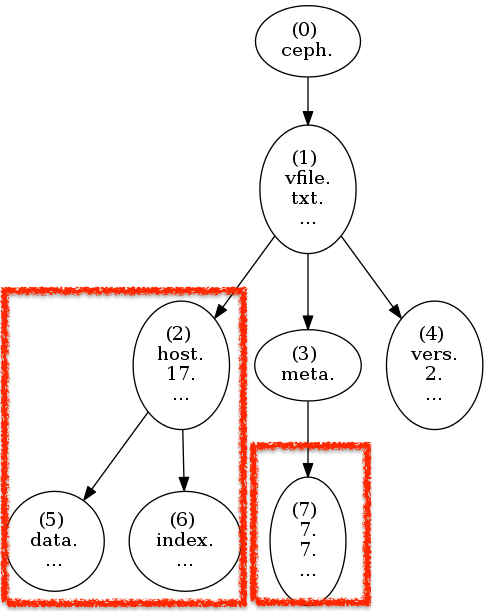
\includegraphics[width=90mm]{figures/tree_plfs.png} 
  \caption{The PLFS file system namespace is structured and predictable; the
  pattern (solid line) is repeated for each hosts. In this case, there are three
  hosts so the pattern is repeated two more times. 
  }\label{fig:tree_plfs}
\end{figure}

\subsubsection{Overhead: Processing RPCs}

When PLFS maps a logical file to many physical files, it deterministically
creates the file system namespace in the backend file system.  For \(n\)
processes on \(m\) servers:

\begin{itemize}
  \item[] \texttt{\# of dirs =} \(m \times \texttt{mkdir()}\)
  \item[] \texttt{\# of file =} \(2n \times \texttt{create()} [+ 2n \times \texttt{lookup()}]\)
  \item[] \texttt{\# of file per dir =} \(n/m\)
\end{itemize}

% How does PLFS create namespaces

\textbf{Metadata Writes}: the number of directories is dependent on the number
of PLFS servers. When a file is created in a PLFS mount, a directory called a
container is created in the underlying file system. Inside the container,
directories are created per server resulting in \(m\) requests. The number of
files is dependendent on the number of PLFS processes. Processes write data and
index files to the directory assigned to their server. The number of requests,
which can range from \(2n\) to \(4n\), is a function of files per directory.
If each server only has one process, then the number of file create requests
will be \(2n\) because each process can cache the directory inode and create
files in one request. With multiple processes per server, clients write to the
same directory and the number of requests doubles because processes cannot
cache the directory inode.

%TODO: multiple processes per node
%TODO: verify path traversal
\begin{figure}[tb]
\centering
  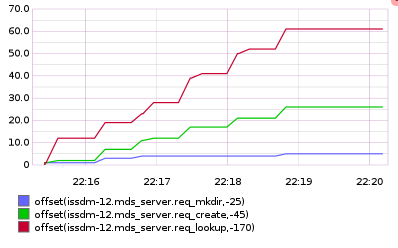
\includegraphics[width=90mm]{figures/prob_reqs.png} 
  \caption{The requests scale linearly with the number of clients.
  \texttt{lookup()} requests dominate because clients share the root and must do
  path traversal.
  }\label{fig:arch}
\end{figure}

% How does PLFS read the namespace
\textbf{Metadata Reads}: transforming write IO in this way has space and read
overheads. In PLFS, this is a problem because index files need to be coalesced
on reads.  Patterned PLFS~\cite{he:hpdc13-plfs-patterns} reduces the space
overheads by storing formulas, instead of index files, to represent write
behavior. Diddlings ~\cite{grider:pc17-diddlings} transfers index files after
each write to absorb the transfer overheads up front. While these approaches
help alleviate read overheads, they do not reduce the file system metadata
load, which is the real problem. Reading the index file still requires a file
system metadata operation.

\begin{itemize}
  \item read file: \(2n \times \texttt{open()}\) 
\end{itemize}

\subsubsection{Microbenchmark}
\subsubsection{Macrobenchmark}

\subsection{ROOT (HEP)}

% the data
The High Energy Physics (HEP) community uses a framework called ROOT to
manipulate, manage, and visualize data about proton-proton collisions
collected at the large hadron collider (LHC). The data is used to re-simulate
phenomena of interest for analysis and there are different types of
reconstructions each with various granularities. The data is organized as
nested and object oriented event data and the length of the runs (and thus
the number of events) are of arbitrary length and type ({\it e.g.},
particle objects, records of low-level detector hit properties).
Reconstruction takes detector conditions ({\it e.g.}, alignment, position of
the beam, etc.) as input, which is pulled from remote database.  Data is
streamed from the LHC into large immutable datasets, stored publicly in
data centers around the world.  Physicists search the dataset and download
interesting events, which are stored as ROOT files. 

\subsubsection{System Architecture}

% WHat does ROOT have?
The advantages of the ROOT framework is the ability to (1) read only parts
of the data and (2) easily ingest remote data over the network. The
disadvantage of the ROOT framework and ROOT files have no formal
specification. Much of the development was done at CERN in parallel with
other HPC ventures. As a result, the technology and strategies are similar
to existing systems:

\begin{itemize}

  \item subdirectories within a file, for organization like HDF5

  \item serialization of any type of C++ object, like Python's pickle, but for
  C++

  \item embedded schema with schema evolution like Avro

  \item columnar storage of large sets of events, like the Dremel/Parquet
  shredding algorithm (called "splitting" in ROOT)

  \item selective reading, also like Dremel/Parquet (the "prune" feature of
  SparkSQL DataFrames)

  \item mutable content; a ROOT file is effectively a single-user object
  database (but without ORM: the data are fundamentally not relational— maybe
  "document store" would be a better word for what it's doing). Not all
  operations are guaranteed to be atomic or thread-safe (hence "single-user").

\end{itemize}

% ROOT files
A ROOT file is a list of objects, accessed by consulting metadata in the
header and seeking to a location in the bytestream. Types of objects include: 

\begin{itemize}

  \item TDirectory: collection of TKeys

  \item TKey: object metadata containing name, title, classname, and seek
  position

  \item TTree: table of a collection of events, listed sequentially and stored in a flat namespace

  \item TBranch: data container representing column(s) of TTree

  \item TLeaf: data type description, stored as a special TBranch member
  that describes the TBranch's data type

  \item TBasket: byte ranges partitioned by events and indexed by TKeys;
  also the compression, parallelization, and tranfer unit

\end{itemize}

The \texttt{splitlevel} parameter controls the data layout, {\it i.e.}
whether it is organized more closely to rowwise or columnar. Low values
store columns values as tuples in entries ({\it i.e.} \texttt{splitlevel=0}
stores all column values as tuples in each entry) while high values make
the data more columnar-based. Other parameters control the size and shape
of hierarchical structure of the ROOT file include events per file, target
TBasket size, cluster size, compression algorithm and level, and alignment
of objects with disk pages.

The ROOT framework uses flat, self-describing files and events are
encoded/de-encoded with three pieces of information: TStreamerInfo to
deserialize bytes, the TBranches hierarchy which describes how columns were
split, and the TLeaves which specify the data types of objects. i

\subsubsection{Namespace Description}

At the top of the namespace of a typical ROOT file there are TKeys, each
containing pointers to groups of TBranches. For example, ``MetaData" has data
about the run and ``Events" has all the proton-proton activity. Logically,
physicists ask for TBranch's so partitioning the ROOT file at this granularity
would prevent read amplification, {\it i.e.} reading more than is necessary.

Unfortunately, the high energy physics community is running into scalability
problems.  The current effort is to integrate the ROOT framework into
CephFS~\cite{weil:osdi2006-ceph}.  Storing ROOT files as objects in an object
store has overhead when users pull the entire GB-sized blob to their laptop.
This model is a mismatch to the workload, which reads metadata and branches
a-la-cart. Partitioning the ROOT file into branches on the file system
namespace allows users to request only the metadata and branches they need.
Unfortunately, storing this metadata in a file system would overwhelm most file
systems because there are too many branches to create a file for each and there
is not enough metadata to reconstruct which branches belong to which events.
Unfortunately, current file system do not have this many inodes and this setup
would require extra metadata to combine TBranches into objects.

\subsubsection{Overheads}

We benchmark the write and read overhead of storing a ROOT file as:

\begin{enumerate}
  \item a large object in Ceph's object store (RADOS)
  \item a large object in RADOS with push-down logic (CLS)
  \item files in Ceph's file system (CephFS)
\end{enumerate}

Setups 1 and 2 are deployed without any changes to the ROOT framework. For
setup 3, TBaskets are stored in Ceph objects and the TBranch hierarchy,
TStreamInfo metadata, and TLeaf metadata map onto the metadata server.
Clients contact the metadata server with a TBranch request, receive back
the TBranch hierarchy necessary to name the Ceph object containing the TBasket
as well as the TStreamInfo and TLeaf metadata necessary to read the object. 

The workload is a list of branch accesses from a trace of the NPTupleMaker high
energy physics application. Each branch access is:

\noindent\texttt{branch0 branch1 ,3,1740718587,5847,97,136}

Where the tuple is full branch name, basket number, offset into the ROOT file,
size of the basket, start of entry of the basket, and end entry of the basket.
For setups 1 and 2 we care about offset into the ROOT file and the size of the
basket.  In setup 1, the ROOT file is pulled locally and the branches are read
from the file. In setup 2, the offset and size of the read are sent as filters
to the OSDs; think of them as push-down predicates from the database world.
For setup 3, we care about the full branch name and basket number.  In setup 3,
the branch accesses are specified as full branch names ({\it i.e.} full path
names), which are used to traverse the file system namespace. The start and end
entry of the basket are the logical records that bookend the basket ({\it
e.g.}, for a start entry of 10 and end entry of 20 for a basket storing user
ages, the start entry is user 10's age and the end entry is user 20's age).  

\subsection{SIRIUS (HPC)}
